% Final report (Phase II) - IEEE conference format
% Build:  pdflatex report_final.tex   (run twice; needs datapath.pdf and waves/ in this folder)
\documentclass[conference]{IEEEtran}
\usepackage{graphicx}
\usepackage{booktabs}
\usepackage{array}
\usepackage{cite}
\usepackage{url}

\begin{document}

\title{Design and Verification of a Single-Cycle RV32I Processor in Verilog\\
{\large Final Report --- CSA-222 Modern Computer Architecture}}

\author{\IEEEauthorblockN{Rishi Raj (2401010380), Yash Yadav (2401010514), Aditya Samadhiya (2401010037),\\
Kaustubh Ranjan Mishra (2401020116) and Yash Raj (2401010514)}
\IEEEauthorblockA{B.Tech Computer Science and AI, Batch 2024\\
Newton School of Technology, Rishihood University\\
Sonipat, Haryana, India}}

\maketitle

\begin{abstract}
This report presents a compact single-cycle processor that executes a
ten-instruction subset of the RISC-V RV32I base instruction set: ADD, SUB,
AND, OR, XOR, ADDI, LW, SW, BEQ and BNE. The processor is written in
synthesizable Verilog as eleven small modules that mirror the textbook
datapath. It is verified with eight self-checking testbenches and four
hand-assembled programs, two of which target corner cases such as signed
overflow, immediates at their limits, writes to register \texttt{x0} and
branches in every direction; all 169 checks pass in simulation. The design
was synthesized for a Lattice ECP5 FPGA with an open-source tool flow. It
uses 1772 four-input look-up tables and 32 flip-flops, about 7\% of the
device, and reaches a maximum clock frequency of 52.8~MHz. The critical path
is the conditional branch, 18.9~ns from the program counter through the
instruction memory, register file, ALU and zero detection back to the
program counter, with the load path close behind at 17.9~ns. Synthesis also
exposed a memory initialization fault that simulation could not show. The
design has not been run on a physical board.
\end{abstract}

\begin{IEEEkeywords}
RISC-V, RV32I, single-cycle processor, datapath, control unit, Verilog, FPGA
synthesis, static timing analysis
\end{IEEEkeywords}

% ---------------------------------------------------------------------------
\section{Introduction}
Every program eventually runs as a sequence of fetch, decode and execute steps
on a processor. The simplest hardware that can do this is the single-cycle
processor, in which each instruction completes within one clock period. It is
not how fast commercial processors are built, but every later idea in the
course, including pipelining, hazards and forwarding, is a modification of
this design, so building it is the most direct way to understand the others.

We chose RISC-V as the instruction set because it is an open standard, its
base integer subset is small, and its instruction formats were designed to
make decoding simple. The course labs introduce datapaths through MIPS32;
RISC-V follows the same load-store philosophy, so the concepts carry over
directly while the encoding details are new.

The project delivers a working processor with RTL, testbenches, waveforms,
test programs and a synthesis report. Phase I covered the design, the RTL for
every module and simulation of the integrated processor. Phase II, reported
here in full, adds corner-case test programs, synthesis for an FPGA, timing
analysis and a discussion of what the results say about single-cycle design.

% ---------------------------------------------------------------------------
\section{Literature Review}

\subsection{RISC and the RISC-V instruction set}
Patterson and Ditzel argued in 1980 that a small set of simple, regular
instructions leads to simpler hardware and a shorter design time than a large
complex instruction set \cite{patterson1980}. RISC-V, started at UC Berkeley
in 2010, applies that idea as a free and open standard \cite{asanovic2014}.
The specification defines a small base integer ISA, RV32I, and keeps
everything else (multiplication, floating point, compressed instructions) in
optional extensions \cite{riscvspec}. RV32I has 32 registers of 32 bits with
\texttt{x0} fixed at zero, fixed 32-bit instructions, and a handful of
formats in which the register fields and the sign bit of the immediate always
sit in the same bit positions. These choices matter for this project: the
register file can be read before the instruction type is known, and sign
extension always uses bit~31.

\subsection{Textbook single-cycle designs}
Patterson and Hennessy develop a single-cycle datapath step by step for a
subset of load, store, arithmetic-logical and branch instructions, and
introduce the two-level control scheme in which a main decoder produces a
2-bit ALU operation class and a second small decoder turns it into the exact
ALU function \cite{patterson2020}. Harris and Harris present a similar
RISC-V single-cycle processor and give complete HDL for it
\cite{harris2021}. Both texts point out the main weakness of the approach:
the clock period has to fit the slowest instruction, the load, so every other
instruction wastes time. This is the motivation for multi-cycle and pipelined
designs, which are outside the scope of this project. Nisan and Schocken take
the same build-it-from-small-parts approach from logic gates up to a complete
computer \cite{nisan2021}, which influenced how we split the work into small
independently testable modules.

\subsection{Open-source RISC-V cores}
Several open cores show what the design space looks like beyond the textbook.
PicoRV32 is a size-optimized multi-cycle core that trades cycles per
instruction for a small area and a high clock frequency \cite{picorv32}. SERV
goes further and processes data one bit at a time to minimize area
\cite{serv}. Ibex is a production-quality two-stage pipelined core with
extensive verification \cite{ibex}. These cores optimize for area,
frequency or robustness and are correspondingly harder to read. Our design
optimizes for clarity instead: one module per block of the datapath diagram,
no pipelining, and only the instructions needed to demonstrate arithmetic,
memory access and control flow.

\subsection{Tools}
The design is simulated with Icarus Verilog \cite{iverilog} and waveforms are
viewed in GTKWave \cite{gtkwave}, the same tool flow used in the course labs.
For synthesis we use Yosys \cite{yosys} and for placement, routing and static
timing analysis nextpnr \cite{nextpnr}. Together they form a complete
open-source flow from Verilog to a placed and routed FPGA design, which lets
every team member reproduce the results without a vendor licence.

% ---------------------------------------------------------------------------
\section{Proposed Solution}

\subsection{Instruction subset}
Table~\ref{tab:instr} lists the ten supported instructions. They cover four
of the RV32I formats. R-type instructions operate on two registers. I-type
instructions (ADDI and LW) take one register and a 12-bit immediate. The
S-type store splits its immediate across two fields so that the register
fields stay in place. The B-type branches encode a 13-bit offset whose lowest
bit is always zero.

\begin{table}[!htb]
\caption{Supported instructions and their encodings}
\label{tab:instr}
\centering
\begin{tabular}{llccc}
\toprule
Instr. & Format & opcode & funct3 & funct7 \\
\midrule
ADD  & R & 0110011 & 000 & 0000000 \\
SUB  & R & 0110011 & 000 & 0100000 \\
AND  & R & 0110011 & 111 & 0000000 \\
OR   & R & 0110011 & 110 & 0000000 \\
XOR  & R & 0110011 & 100 & 0000000 \\
ADDI & I & 0010011 & 000 & --- \\
LW   & I & 0000011 & 010 & --- \\
SW   & S & 0100011 & 010 & --- \\
BEQ  & B & 1100011 & 000 & --- \\
BNE  & B & 1100011 & 001 & --- \\
\bottomrule
\end{tabular}
\end{table}

\begin{figure*}[t]
\centering
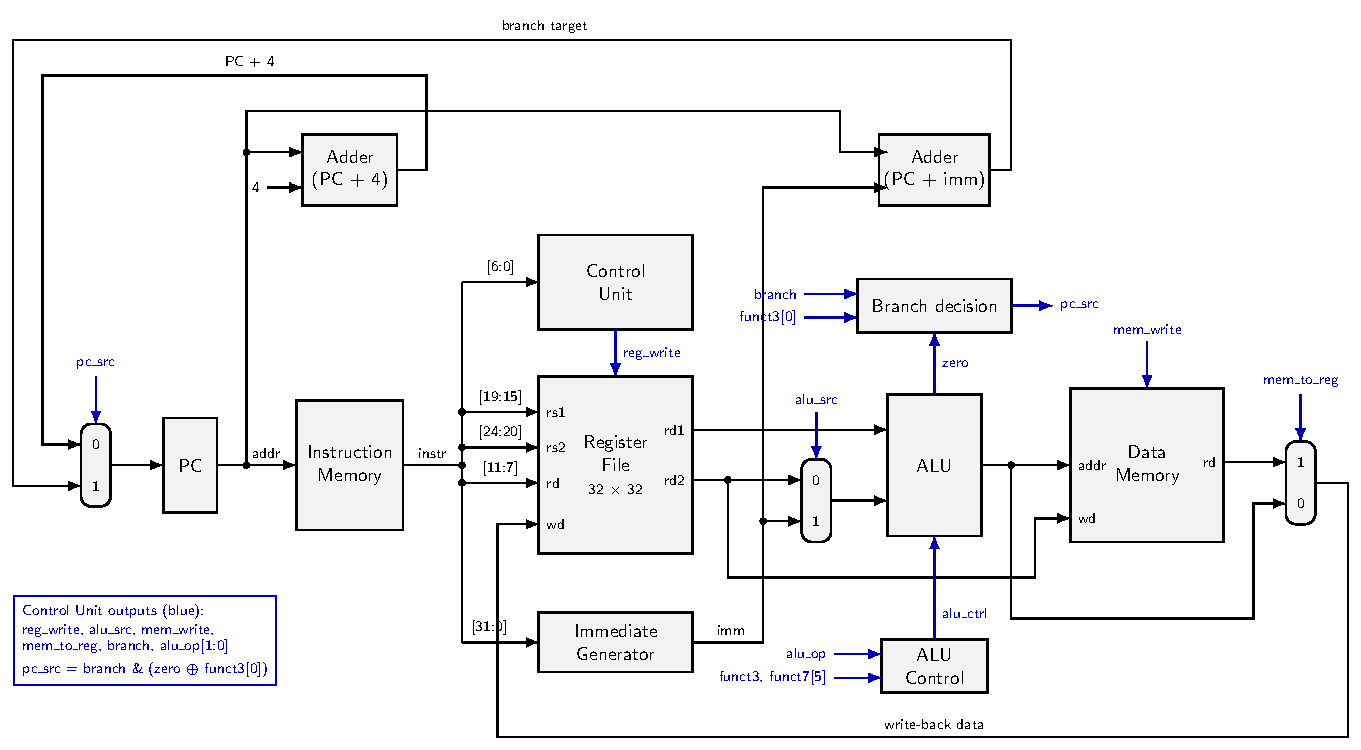
\includegraphics[width=0.95\textwidth]{datapath.pdf}
\caption{Datapath of the single-cycle RV32I processor. Data signals are drawn
in black and control signals in blue.}
\label{fig:datapath}
\end{figure*}

\subsection{Datapath}
Fig.~\ref{fig:datapath} shows the datapath. One instruction moves through it
from left to right in a single clock cycle.

\textit{Fetch.} The program counter (PC) holds the address of the current
instruction. The instruction memory is read combinationally, and an adder
computes PC\,+\,4.

\textit{Decode.} The opcode goes to the control unit. The \texttt{rs1} and
\texttt{rs2} fields address the register file, which returns both values
combinationally. The immediate generator extracts and sign-extends the
immediate according to the instruction format.

\textit{Execute.} A multiplexer selects either the second register value or
the immediate as the second ALU operand. The ALU adds, subtracts or performs
AND, OR or XOR, and raises a \texttt{zero} flag when the result is zero. A
second adder computes the branch target PC\,+\,immediate.

\textit{Memory.} For LW and SW the ALU result is the memory address. Data
memory is read combinationally and written on the clock edge.

\textit{Write-back.} A multiplexer selects the ALU result or the memory data
and sends it back to the register file, which is written on the clock edge.

Only three things change on the clock edge: the PC, one register and one
memory word. Everything else is combinational logic, which is what makes the
design single-cycle.

\subsection{Control}
Control is split into two levels, following \cite{patterson2020}. The main
control unit looks only at the opcode and produces the signals in
Table~\ref{tab:control}. The ALU control block then uses the 2-bit
\texttt{alu\_op} together with \texttt{funct3} and bit 5 of \texttt{funct7}
to pick the ALU operation. ADD and SUB differ only in that \texttt{funct7}
bit; for ADDI the same bit position belongs to the immediate, so subtraction
is selected only when the opcode is R-type.

Branches reuse the ALU: it subtracts the two registers, and
\texttt{zero}\,=\,1 means they are equal. BEQ and BNE differ only in
\texttt{funct3[0]}, so the next-PC select is
\[
\texttt{pc\_src} = \texttt{branch} \cdot (\texttt{zero} \oplus \texttt{funct3[0]}).
\]
An unknown opcode leaves every write enable at zero, so it cannot corrupt
registers or memory.

\begin{table}[!htb]
\caption{Main control unit truth table (x = don't care)}
\label{tab:control}
\centering
\setlength{\tabcolsep}{3.5pt}
\begin{tabular}{lcccccc}
\toprule
Class & \rotatebox{70}{reg\_write} & \rotatebox{70}{alu\_src} &
\rotatebox{70}{mem\_write} & \rotatebox{70}{mem\_to\_reg} &
\rotatebox{70}{branch} & \rotatebox{70}{alu\_op} \\
\midrule
R-type    & 1 & 0 & 0 & 0 & 0 & 10 \\
ADDI      & 1 & 1 & 0 & 0 & 0 & 10 \\
LW        & 1 & 1 & 0 & 1 & 0 & 00 \\
SW        & 0 & 1 & 1 & x & 0 & 00 \\
BEQ / BNE & 0 & 0 & 0 & x & 1 & 01 \\
\bottomrule
\end{tabular}
\end{table}

\subsection{RTL structure}
Each block in Fig.~\ref{fig:datapath} is one Verilog module: \texttt{pc},
\texttt{adder}, \texttt{instr\_mem}, \texttt{control\_unit},
\texttt{reg\_file}, \texttt{imm\_gen}, \texttt{alu\_control}, \texttt{alu},
\texttt{mux2}, \texttt{data\_mem}, and the top level \texttt{rv32i\_top}
which only wires them together. Both memories hold 64 words. The instruction
memory is initialized from a hex file with \texttt{\$readmemh}, so a new
program can be run without touching the RTL. Programs are written in RISC-V
assembly and assembled by hand into hex; each hex line carries the assembly
as a comment.

\subsection{Verification approach}
Every module has a self-checking testbench that applies inputs, compares the
outputs against expected values and prints a pass or fail summary. A failing
run also ends with a non-zero exit status, so a script cannot mistake it for
a pass. The integrated processor is tested by running complete programs: the
testbench loads a hex file, runs until the program reaches its halt
instruction (a branch to itself), counts the clock cycles and then compares
the final registers and memory with values worked out by hand. The results
are given in Section~\ref{sec:results}.

% ---------------------------------------------------------------------------
\section{Results and Discussion}
\label{sec:results}

\subsection{Functional verification}
Table~\ref{tab:tests} lists the testbenches. All 169 checks pass in Icarus
Verilog. Phase II added the limits of every immediate field to
\texttt{tb\_imm\_gen}, including the farthest forward and backward branch
offsets of $+4094$ and $-4096$ bytes, and values at the edges of the 32-bit
range to \texttt{tb\_alu}.

\begin{table}[!htb]
\caption{Testbenches and number of checks}
\label{tab:tests}
\centering
\begin{tabular}{@{}l>{\raggedright\arraybackslash}p{4.3cm}c@{}}
\toprule
Testbench & What is checked & Checks \\
\midrule
\texttt{tb\_fetch}   & reset, PC\,+\,4 stepping, jump to target, instruction read & 7 \\
\texttt{tb\_reg\_file} & write and read, dual read ports, write enable, \texttt{x0} stays zero & 10 \\
\texttt{tb\_imm\_gen} & I, S and B immediates, including the limits of each field & 23 \\
\texttt{tb\_alu}     & five ALU operations, zero flag, overflow and wraparound, ALU decoder & 36 \\
\texttt{tb\_control\_unit} & control table, unknown opcodes, multiplexer & 9 \\
\texttt{tb\_data\_mem} & write and read back, write enable, address range & 9 \\
\texttt{tb\_rv32i\_top} & final state of four programs & 55 \\
\texttt{tb\_fpga\_top} & LED output of the board wrapper & 20 \\
\midrule
Total & & 169 \\
\bottomrule
\end{tabular}
\end{table}

Table~\ref{tab:programs} lists the four test programs. Programs 1 and 2 are
from Phase I. Program 3 targets the datapath: the largest and smallest ADDI
immediates, two writes and one load into \texttt{x0}, the constant
\texttt{0x80000000} built by doubling 1 thirty-one times (the subset has no
LUI), signed overflow in both directions, and stores and loads with a
negative offset and at the last word of data memory. Program 4 targets
control flow and checks itself: each of eight branch checks that behaves
correctly adds one to \texttt{x31}, and every instruction that should be
skipped adds one to \texttt{x30}. It covers BEQ and BNE taken and not taken,
equal negative operands, a forward branch over a block followed by a backward
branch into it, a nested loop that computes $6 \times 7$, and a branch on a
value loaded from memory. It finishes with \texttt{x31}\,=\,8 and
\texttt{x30}\,=\,0.

\begin{table}[!htb]
\caption{Test programs. Cycles are counted up to the halt instruction and
equal the number of instructions executed.}
\label{tab:programs}
\centering\setlength{\tabcolsep}{4pt}
\begin{tabular}{@{}l>{\raggedright\arraybackslash}p{3.0cm}ccc@{}}
\toprule
Program & Purpose & Size & Cycles & Result \\
\midrule
\texttt{prog1\_arith}  & arithmetic, logic, load, store & 15 & 14  & pass \\
\texttt{prog2\_loop}   & sum 5 down to 1, branches      & 14 & 24  & pass \\
\texttt{prog3\_corner} & datapath corner cases          & 30 & 119 & pass \\
\texttt{prog4\_branch} & branch corner cases, nested loop & 35 & 169 & pass \\
\bottomrule
\end{tabular}
\end{table}

To confirm that the new programs can actually detect faults, we broke the
design on purpose in a scratch copy. With the BNE inversion removed from the
branch decision, program 4 reported wrong values in \texttt{x31},
\texttt{x30} and the loop product. With the \texttt{x0} protection removed
from the register file, program 3 failed on the first register that depends
on \texttt{x0}. Both faults were caught.

Table~\ref{tab:results} gives a selection of expected and simulated values.
The corner cases behave as the RISC-V specification requires: arithmetic
wraps around modulo $2^{32}$ with no trap on overflow, \texttt{x0} reads as
zero whatever is written to it, and the immediates are sign-extended at both
limits.

\begin{table}[!htb]
\caption{Selected expected and simulated values}
\label{tab:results}
\centering
\begin{tabular}{@{}llcc@{}}
\toprule
Prog. & Location & Expected & Simulated \\
\midrule
1 & \texttt{x4} (10 $-$ 6)                 & 4  & 4 \\
1 & \texttt{x8} (ADDI $-$3)                & $-$3 & $-$3 \\
1 & \texttt{mem[8]}                        & 20 & 20 \\
2 & \texttt{x2} (loop sum)                 & 15 & 15 \\
3 & \texttt{x4} (after writes to \texttt{x0}) & 0 & 0 \\
3 & \texttt{x8} (\texttt{7FFFFFFF} + 1)    & \texttt{80000000} & \texttt{80000000} \\
3 & \texttt{x11} ($-$2048 $-$ 2047)        & $-$4095 & $-$4095 \\
3 & \texttt{x17} (load at offset $-$4)     & \texttt{7FFFFFFF} & \texttt{7FFFFFFF} \\
3 & \texttt{mem[252]} (last word)          & \texttt{FFFFFFFF} & \texttt{FFFFFFFF} \\
4 & \texttt{x31} (checks passed)           & 8  & 8 \\
4 & \texttt{x30} (skipped code run)        & 0  & 0 \\
4 & \texttt{x12} ($6 \times 7$)            & 42 & 42 \\
\bottomrule
\end{tabular}
\end{table}

\begin{figure*}[t]
\centering
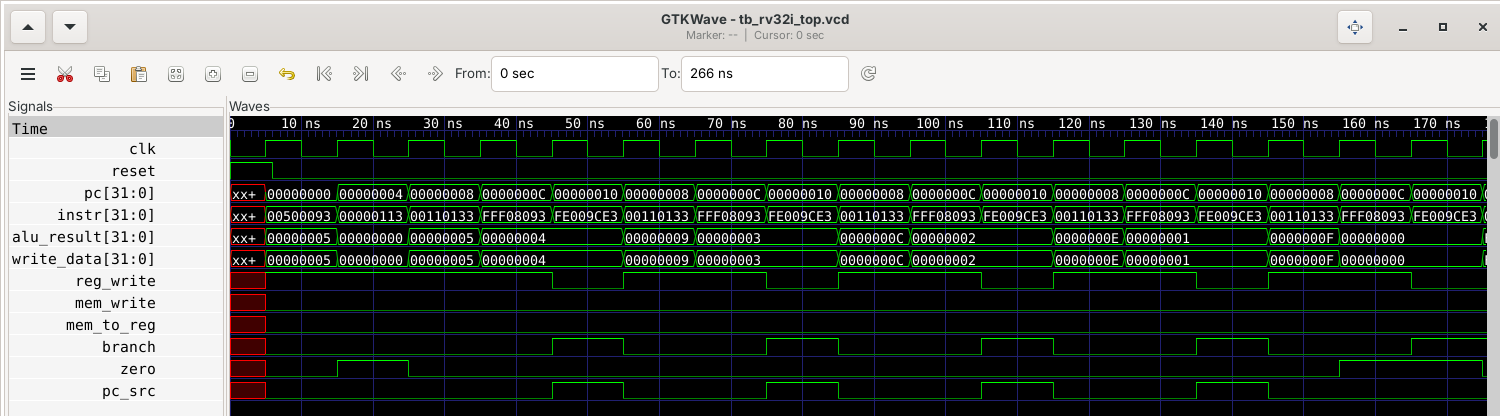
\includegraphics[width=\textwidth]{waves/prog2_loop.png}
\caption{GTKWave trace of program 2. The PC steps 08, 0C, 10 and then
returns to 08: \texttt{branch} and \texttt{pc\_src} go high on the BNE at
address 10 while \texttt{zero} is low, so the branch is taken.}
\label{fig:wave2}
\end{figure*}

\begin{figure*}[t]
\centering
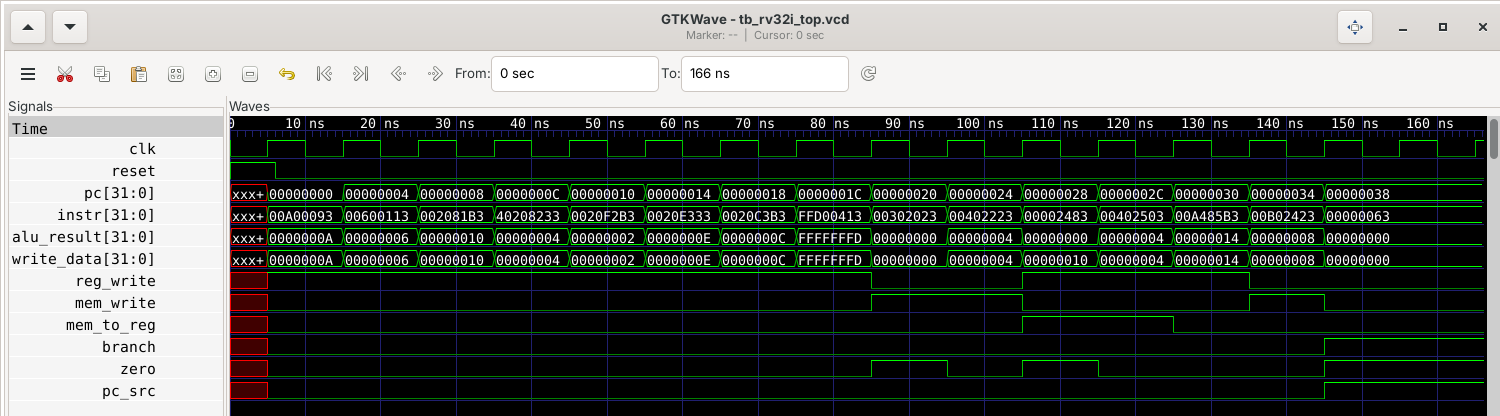
\includegraphics[width=\textwidth]{waves/prog1_arith.png}
\caption{GTKWave trace of program 1. \texttt{mem\_write} is high for the two
SW instructions at addresses 20 and 24, and \texttt{mem\_to\_reg} is high for
the two LW instructions that follow. The PC stops at 38, the halt
instruction.}
\label{fig:wave1}
\end{figure*}

\subsection{Waveform evidence}
Fig.~\ref{fig:wave2} shows the loop of program 2. Each clock period holds one
complete instruction: the PC, the instruction word, the ALU result and the
write-back value all change together on the rising edge. On the BNE at
address \texttt{10} the ALU subtracts \texttt{x0} from the loop counter, the result
is non-zero, and \texttt{pc\_src} selects the branch target so the next PC is
\texttt{08}. Fig.~\ref{fig:wave1} shows program 1, where the control signals
separate the instruction classes: \texttt{reg\_write} is low only for stores
and the final branch, \texttt{mem\_write} is high only for stores, and
\texttt{mem\_to\_reg} is high only for loads.

\subsection{Synthesis and resource usage}
The design was synthesized with Yosys for a Lattice ECP5 LFE5U-25F and placed
and routed with nextpnr. A real program leaves many instruction bits
constant, and the tool would then remove the logic that those bits drive. To
get numbers that do not depend on the program, the instruction memory was
filled with random words for synthesis.

Table~\ref{tab:resources} gives the totals after place and route, and
Table~\ref{tab:modules} splits the logic by module. The design fits in 7\%
of the look-up tables of the device. Only 32 flip-flops are used, all in the
PC, because the register file and data memory map to distributed RAM built
from look-up tables instead of individual flip-flops.

\begin{table}[!htb]
\caption{Resource usage on the ECP5 LFE5U-25F after place and route}
\label{tab:resources}
\centering
\begin{tabular}{@{}lrr@{}}
\toprule
Resource & Used & Available \\
\midrule
Look-up tables (LUT4), total   & 1772 & 24288 \\
\quad logic                    & 1260 & \\
\quad carry chains             & 128  & \\
\quad distributed RAM          & 384  & \\
Flip-flops                     & 32   & 24288 \\
Block RAM                      & 0    & 56 \\
I/O pins                       & 130  & 197 \\
\bottomrule
\end{tabular}
\end{table}

\begin{table}[!htb]
\caption{Logic by module after synthesis}
\label{tab:modules}
\centering
\begin{tabular}{@{}lrl@{}}
\toprule
Module & Logic LUT4 & Other cells \\
\midrule
\texttt{reg\_file}      & 517 & 32 RAM cells \\
\texttt{alu}            & 283 & 32 carry cells \\
\texttt{data\_mem}      & 132 & 32 RAM cells \\
\texttt{instr\_mem}     & 128 & \\
\texttt{mux2} ($\times 3$) & 96 & \\
\texttt{control\_unit}  & 52  & \\
\texttt{imm\_gen}       & 40  & \\
\texttt{alu\_control}   & 11  & \\
\texttt{adder} ($\times 2$) & 0 & 32 carry cells \\
\texttt{pc}             & 0   & 32 flip-flops \\
top-level glue          & 1   & \\
\midrule
Total                   & 1260 & \\
\bottomrule
\end{tabular}
\end{table}

The register file is the largest block, with 41\% of the logic. The storage
itself is cheap; the cost is in the two read ports. Each output bit selects
between the two halves of the memory and is forced to zero when the address
is \texttt{x0}, which makes it a function of seven inputs. The default
mapping builds every such function from eight four-input tables and a tree
of multiplexers, so 64 output bits cost about 512 tables. Re-running
synthesis with the newer \texttt{abc9} mapper reduced the logic from 1260 to
877 tables at a similar clock frequency, which shows how much of the area is
decided by the tool and not by the RTL. The reported numbers use the default
flow.

\textit{A fault found by synthesis.} In the first synthesis run the
instruction memory came out empty. The RTL cleared the memory in a loop and
then loaded the program with \texttt{\$readmemh}. Simulators run these in
order, but Yosys applied the clearing loop last and the result was a ROM of
zeros. Every simulation passed, yet the processor would have executed
nothing on hardware. The clearing loop is now compiled only for simulation.
This was the most useful single result of Phase II: passing simulation does
not prove that the synthesized circuit matches the RTL.

\subsection{Timing and critical path}
nextpnr reports a maximum clock frequency of 52.8~MHz, a minimum period of
18.9~ns, for speed grade 6. Five runs with different placement seeds gave
51.5 to 52.8~MHz. Of the 18.9~ns, 7.0~ns is logic delay and 11.9~ns is
routing, so wires account for 63\% of the cycle.

The critical path is a conditional branch. Table~\ref{tab:path} follows it
from the PC through every block of the datapath and back to the PC. The
subtraction in the ALU and the 32-bit zero detection after it are the two
largest contributions.

\begin{table}[!htb]
\caption{Critical path (branch) by stage}
\label{tab:path}
\centering
\begin{tabular}{@{}lrr@{}}
\toprule
Stage & Delay (ns) & Arrival (ns) \\
\midrule
PC register, clock to output      & 0.5 & 0.5 \\
Instruction memory                & 2.0 & 2.5 \\
Register file read                & 3.2 & 5.7 \\
ALU source multiplexer            & 1.7 & 7.4 \\
ALU subtract                      & 5.0 & 12.4 \\
Zero detection                    & 3.5 & 15.9 \\
Branch decision (\texttt{pc\_src}) & 1.4 & 17.3 \\
PC multiplexer                    & 1.5 & 18.8 \\
PC register setup                 & 0.1 & 18.9 \\
\bottomrule
\end{tabular}
\end{table}

The textbooks name the load as the slowest instruction of a single-cycle
processor \cite{patterson2020, harris2021}, so we measured that path as well.
The timing tool reports only the longest path, so in a scratch copy we tied
the branch select to zero and repeated the flow. The longest remaining path
was the load, at 17.9~ns: PC, instruction memory, register file, ALU, data
memory (3.6~ns), write-back multiplexer and the register file write port. In
our design the branch is therefore about 1~ns slower than the load. The
reason is the size of the memories. A 64-word data memory built from
look-up tables is read in 3.6~ns, which is about what the zero detection
costs, and the branch then still has to pass through the branch decision and
the PC multiplexer. With a data memory of realistic size the read would take
far longer and the load would be the critical path, as the textbooks say.

\subsection{Performance observations}
Every instruction takes exactly one cycle, so the cycles per instruction
(CPI) is 1 and the execution time is the instruction count multiplied by the
clock period. At the minimum period of 18.9~ns, program 1 takes
0.26~$\mu$s, program 2 takes 0.45~$\mu$s, program 3 takes 2.25~$\mu$s and
program 4 takes 3.19~$\mu$s.

The weakness of the design is visible in the two path measurements. Every
instruction is given 18.9~ns because the branch needs it. An ADD uses
neither the data memory nor the branch logic; taking the load path without
the data memory read as a rough estimate, it would be finished after about
14~ns and then waits. A single-cycle processor cannot give different
instructions different amounts of time, because there is one clock and no
state between the stages. A pipelined design removes this limit by placing
registers between the stages so that the clock period is set by the slowest
stage instead of the whole path. From Table~\ref{tab:path} the slowest
stage here would be the execute stage at roughly 7 to 9~ns depending on
where the registers are placed, which suggests about twice the clock
frequency before hazards are taken into account. We did not build this; it
is the natural next step.

\subsection{FPGA deployment and limitations}
No FPGA board was available, so the design has not been run on hardware and
the timing numbers come from static analysis after place and route, not
from measurement. To make deployment straightforward we added a board
wrapper, \texttt{fpga\_top}, that divides the board clock down to a few
hertz and shows the instruction index on eight LEDs. The wrapper is
simulated by its own testbench and synthesizes without errors.

Other limitations: the processor implements ten instructions, with no
jumps, shifts, comparisons, upper-immediate or byte and half-word memory
accesses; both memories hold 64 words; and the instruction memory is fixed
at synthesis time. There are no interrupts or exceptions, and an unknown
opcode is silently ignored.

% ---------------------------------------------------------------------------
\section{Individual Contributions}
Each member owns a part of the datapath together with its testbench, and in
Phase II one part of the evaluation work. Table~\ref{tab:contrib} lists the
split. The demonstration video is available online at
\url{https://drive.google.com/file/d/1IhI9AuI-NJyWOLgHf0MOzuwAFhSgHOxk/view?usp=sharing}.

\begin{table}[!htb]
\caption{Individual contributions}
\label{tab:contrib}
\centering
\setlength{\tabcolsep}{3pt}
\begin{tabular}{@{}>{\raggedright\arraybackslash}p{1.9cm}>{\raggedright\arraybackslash}p{2.7cm}>{\raggedright\arraybackslash}p{3.6cm}@{}}
\toprule
Member & Phase I & Phase II \\
\midrule
Rishi Raj\newline(2401010380) &
  \texttt{pc}, \texttt{adder}, \texttt{instr\_mem}, \texttt{tb\_fetch}; programs 1 and 2 &
  Corner-case programs 3 and 4, hand-assembled; instruction memory fix for synthesis.
  \emph{Report:} Abstract, Introduction, program results \\
\addlinespace
Yash Yadav\newline(2401010514) &
  \texttt{reg\_file}, \texttt{imm\_gen} and their testbenches &
  Immediate limit tests; GTKWave capture script and waveform figures.
  \emph{Report:} Literature Review, waveform evidence \\
\addlinespace
Aditya Samadhiya\newline(2401010037) &
  \texttt{alu}, \texttt{alu\_control}, \texttt{tb\_alu}; block diagram &
  ALU corner-case tests; synthesis script and resource report.
  \emph{Report:} Datapath, synthesis and resource usage \\
\addlinespace
Kaustubh Ranjan Mishra\newline(2401020116) &
  \texttt{control\_unit}, \texttt{mux2}, \texttt{tb\_control\_unit} &
  Place and route; critical path, load path and clock frequency analysis.
  \emph{Report:} Control, timing and performance \\
\addlinespace
Yash Raj\newline(2401010514) &
  \texttt{data\_mem}, \texttt{rv32i\_top}, their testbenches; repository &
  Four-program top-level testbench; FPGA wrapper and its testbench; build flow.
  \emph{Report:} Verification, limitations, Conclusion \\
\bottomrule
\end{tabular}
\end{table}

% ---------------------------------------------------------------------------
\section{Conclusion}
We designed a single-cycle RV32I processor in Verilog, one module per block
of the datapath, and verified it with 169 checks across eight testbenches
and four hand-assembled programs. The corner-case programs confirmed
wraparound arithmetic, the hardwired zero register, sign extension at the
limits of every immediate field and correct branching in every direction.
Synthesized for a Lattice ECP5, the processor uses 1772 look-up tables and
32 flip-flops and runs at up to 52.8~MHz.

Three results go beyond a working simulation. First, synthesis exposed a
memory initialization fault that no testbench could see, which is a concrete
reason to synthesize early. Second, the critical path in our design is the
branch and not the load, because the memories are small; which instruction
is slowest depends on the implementation and not only on the architecture.
Third, most of the clock period is routing delay and most of the area is in
the read multiplexers of the register file, neither of which is visible in
the RTL.

The design has not been tested on a board, and it covers only ten
instructions. The next steps would be running it on an FPGA, adding the
remaining RV32I instructions, and pipelining the datapath, which the timing
breakdown suggests could roughly double the clock frequency.

% ---------------------------------------------------------------------------
\begin{thebibliography}{00}
\bibitem{patterson1980} D. A. Patterson and D. R. Ditzel, ``The case for the
reduced instruction set computer,'' \emph{ACM SIGARCH Comput. Archit. News},
vol. 8, no. 6, pp. 25--33, Oct. 1980.
\bibitem{asanovic2014} K. Asanovi\'c and D. A. Patterson, ``Instruction sets
should be free: The case for RISC-V,'' EECS Dept., Univ. California, Berkeley,
Tech. Rep. UCB/EECS-2014-146, Aug. 2014.
\bibitem{riscvspec} A. Waterman and K. Asanovi\'c, Eds., \emph{The RISC-V
Instruction Set Manual, Volume I: Unprivileged ISA}, Document Version
20191213, RISC-V Foundation, Dec. 2019.
\bibitem{patterson2020} D. A. Patterson and J. L. Hennessy, \emph{Computer
Organization and Design RISC-V Edition: The Hardware Software Interface},
2nd ed. Cambridge, MA, USA: Morgan Kaufmann, 2020.
\bibitem{harris2021} S. L. Harris and D. M. Harris, \emph{Digital Design and
Computer Architecture: RISC-V Edition}. Cambridge, MA, USA: Morgan Kaufmann,
2021.
\bibitem{nisan2021} N. Nisan and S. Schocken, \emph{The Elements of Computing
Systems: Building a Modern Computer from First Principles}, 2nd ed.
Cambridge, MA, USA: MIT Press, 2021.
\bibitem{picorv32} C. Wolf, ``PicoRV32: A size-optimized RISC-V CPU.''
[Online]. Available: \url{https://github.com/YosysHQ/picorv32}
\bibitem{serv} O. Kindgren, ``SERV: The serial RISC-V CPU.'' [Online].
Available: \url{https://github.com/olofk/serv}
\bibitem{ibex} lowRISC, ``Ibex RISC-V core.'' [Online]. Available:
\url{https://github.com/lowRISC/ibex}
\bibitem{iverilog} S. Williams, ``Icarus Verilog.'' [Online]. Available:
\url{https://steveicarus.github.io/iverilog/}
\bibitem{gtkwave} T. Bybell, ``GTKWave.'' [Online]. Available:
\url{https://gtkwave.sourceforge.net/}
\bibitem{yosys} C. Wolf, ``Yosys Open SYnthesis Suite.'' [Online]. Available:
\url{https://yosyshq.net/yosys/}
\bibitem{nextpnr} D. Shah, E. Hung, C. Wolf, S. Bazanski, D. Gisselquist, and
M. Milanovic, ``Yosys+nextpnr: An open source framework from Verilog to
bitstream for commercial FPGAs,'' in \emph{Proc. IEEE Int. Symp.
Field-Programmable Custom Comput. Mach. (FCCM)}, 2019, pp. 1--4.
\end{thebibliography}

\end{document}
